% This is samplepaper.tex, a sample chapter demonstrating the
% LLNCS macro package for Springer Computer Science proceedings;
% Version 2.20 of 2017/10/04
%
\documentclass[runningheads]{llncs}
%
\usepackage{graphicx}
% Used for displaying a sample figure. If possible, figure files should
% be included in EPS format.
%
% If you use the hyperref package, please uncomment the following line
% to display URLs in blue roman font according to Springer's eBook style:
% \renewcommand\UrlFont{\color{blue}\rmfamily}

\begin{document}
%
\title{Direction-Free In-Air Signature Verification Using WIFI CSI Signal}
%
%\titlerunning{Abbreviated paper title}
% If the paper title is too long for the running head, you can set
% an abbreviated paper title here
%
\author{Young Woong KWON\inst{1} \and
JooYoung KIM\inst{1} \and
Kar-Ann TOH\inst{1}}
%
\authorrunning{F. Author et al.}
% First names are abbreviated in the running head.
% If there are more than two authors, 'et al.' is used.
%
\institute{Yonsei University \and
\email{lncs@springer.com}\\
\url{http://www.springer.com/gp/computer-science/lncs} \and
ABC Institute, Rupert-Karls-University Heidelberg, Heidelberg, Germany\\
\email{\{abc,lncs\}@uni-heidelberg.de}}
%
\maketitle              % typeset the header of the contribution
%
\begin{abstract}
The abstract should briefly summarize the contents of the paper in
15--250 words.

\keywords{First keyword  \and Second keyword \and Another keyword.}
\end{abstract}
%
%
%
\section{Introduction}

\subsection{Motivation}
i. Pros of In-Air WIFI CSI signature system
1) Cheap: Use commercial device
2) Easy: No additional devices is needed
3) Secure: Hard to forgery
ii. Cons of In-Air WIFI CSI signature system
1) Setting direction problem
a) Different direction -> Different feature is needed
b) Hard to set exactly same direction as authentication before
Size of signature can varies

\subsection{Contribution}
- Overcome cons of WIFI signature system
- Robust to signal direction, size

\section{Related Works}
a. WIFI CSI
b. Siamese Networks

\subsection{WIFI CSI}
- An In-Air Signature Verification System Using Wi-Fi Signals 

\section{Proposed System}

%system overview
In this section, we introduce a system for recognition of Wi-Fi based in-air signature which utilizes the Siamese network learning for validation.
An overview of the proposed scheme is shown in Fig.1.
% main purpose
The main purpose of this system is to receive two csi signals as input, to 
determine if the two signals are the same signature.
Since signals may differ in the direction in which they are entered, our system must be capable of extracting non-direction-related characteristics from two signals.
% Figure 1
\begin{figure}
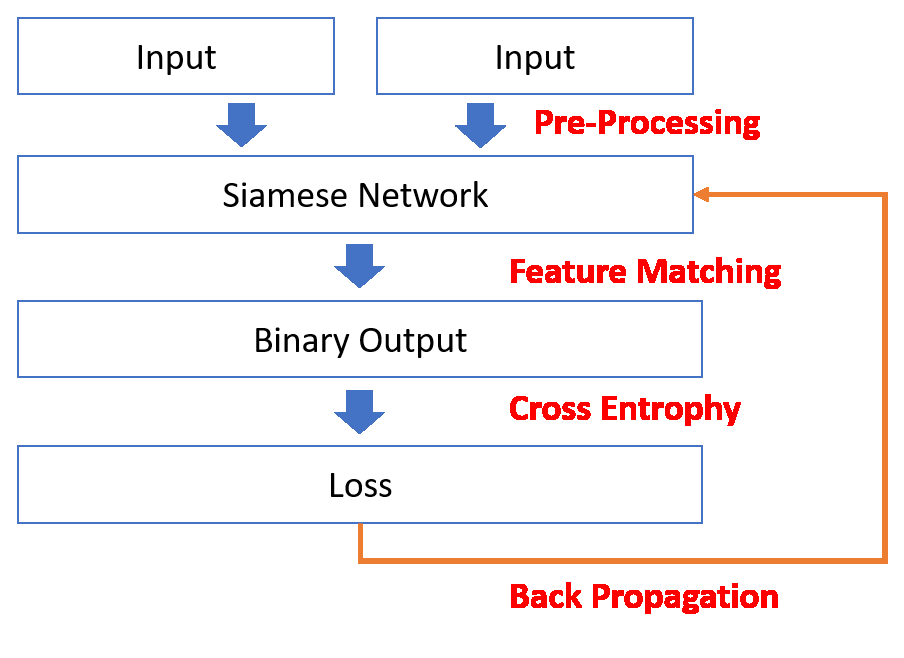
\includegraphics[width=\textwidth]{methods1.eps}
\caption{...} \label{method1}
\end{figure}

\subsection{Data Preprocessing}
% preprocessing
In order to be used as an input to a siamese network, the signal must be pre-processed.

First, the signal have to be converted to non-complex form.
Since the Wi-Fi signature signals in CSI packets in 2.4Ghz has firmware issues in their phase[ref]. so we used absolute of signal only.

% From HC's Papaer
Second, all inputs must be arranged of same size.
Since all signals have different length, the gradient operation with respect to the time instance is adopted to measure the short time energy. 
Data points with the highest short-time energy within the time period are regarded as the starting and the ending points of the in-air signature.
And they are re-sampled uniformly based on Fast Fourier Transform (FFT) [16] to normalize the length of the data. 
% HC's end

% Methods 

\subsection{Siamese Network For Verification}

% Introduce Siamese Net
% From Ref1 start
Siamese nets were first introduced in the early 1990s by Bromley and LeCun to solve signature verification as an image matching problem (Bromley et al., 1993)
Siamese neural networks employ a unique structure to naturally rank similarity between inputs.
It can discriminate between the class-identity of image pairs
The verification model learns to identify input pairs according to the probability that they belong to the same class or different classes.[1]
% From Ref1 End

% Functions of Siamese in our system
The model receives two processed CSI signals as inputs, and outputs the probability that the two signals are of the same class as the output. 
The output of the Siamese network is 1 when the distance of the characteristic vector is close, and 0 when it is far.
the network is learned by the back-propagation.

Two preprocessed signals enter the Siamese network and the network extracts non-directional characteristics from two signals and calculates how similar the two extracted characteristics are.

Even if a signal belongs to the same class, the shape of the input is very different if the signal is oriented differently.
To classify regardless of the direction of the signal, the model shall be capable of extracting features unrelated to the direction.


% Section: Feature Extraction
\subsubsection{Feature Extraction}
When two processed signals come as the input, they are put to 2 symmetric CNN network.

% CNN: purpose
Purpose of CNN is to extract features from signal.
By sharing their feature map, this CNN networks is trainin to learn characteristics regardless of the direction only.

% how to extract feature using CNN
To perform the feature extraction, we firstly need to have a convolutional neural networks  to serve as the feature extractor
Based on the ConvNet structure [17] the feature extractor of the proposed pretraining model consists of i convolution layers and activation functions followed by i max-pooling layers. Each convolution layer has f∗ filters to be trained, where ∗ = 1, ..., i. In a similar manner, j fully connected layers constitute the classifier of pretraining model where each layer has g•,(•=1,...,j) neurons to be trained. 

%Symmetric Architecture
Some of the features CNN extracted are related to the shape of the signature, but CNN's features are not just those that helpful to classify signatures. some may be heavily influenced by the direction in which the signature was entered.
We aim to classify the signature in a direction that is not related to the direction in which it was entered. This type of property interferes with the classification of signatures.

To focus on characteristics conducive to classification, The two CNN networks are arranged side by side symmetrically.
It was also designed to have the same weight on the symmetrical CNN network as on a symmetrical CNN network. 

% tied weights


%Symetric : Share Weights
% To extract the same characteristics from signals in different directions.
% CNN: Feature Extractor
%Automatically extract feature vector from CSI image



\subsubsection{Feature Matching}

% Use L1 distances of Feature vector of 2 input images
% From HC's In-Air paper below:
Let $\mathbf{m}\in{\mathrm{R}}^{d\times1}$ and $\mathbf{n}\in{\mathrm{R}}^{d\times1}$ be feature vectors extracted from two samples.
The L-1 distance between the two features can be calculated as  follows:
Where $\mathbf{p}$ denotes the L-1 distance. In the Siamese networks, this L-1 distance is utilized to match between two feature vectors.

% From HC's End
% From Oneshot paper below
\begin{equation}
    \mathbf{p} = 
    \sigma(\sum_j\alpha_{j}\mid
    \mathbf{m}_{1,L-1}^{(j)} - 
    \mathbf{n}_{1,L-1}^{(j)}\mid)  
\end{equation}
where σ is the sigmoidal
activation function. This final layer induces a metric on the learned feature space of the (L − 1)th hidden layer and scores the similarity between the two feature vec- tors. The αj are additional parameters that are learned by the model during training, weighting the importance of the component-wise distance. This defines a final Lth fully-connected layer for the network which joins the two siamese twins.
% From oneshot end



Output of the CNN are feature vectors extracted from two samples. The Euclidean distance between the two features can be calculated.
In the proposed system, this Euclidean distance is utilized to match between two feature vectors.

\subsubsection{Loss and Backpropagation}
 We impose a regularized cross-entropy objective on our binary classifier.
This objective is combined with standard backpropagation algorithm, where the gradient is additive across the twin networks due to the tied weights.
 We initialized all network weights in the convolutional layers from a normal distribution with zero-mean and a standard deviation of 10−2. Biases were also initialized from a normal distribution, but with mean 0.5 and standard deviation 10−2.
\begin{figure}
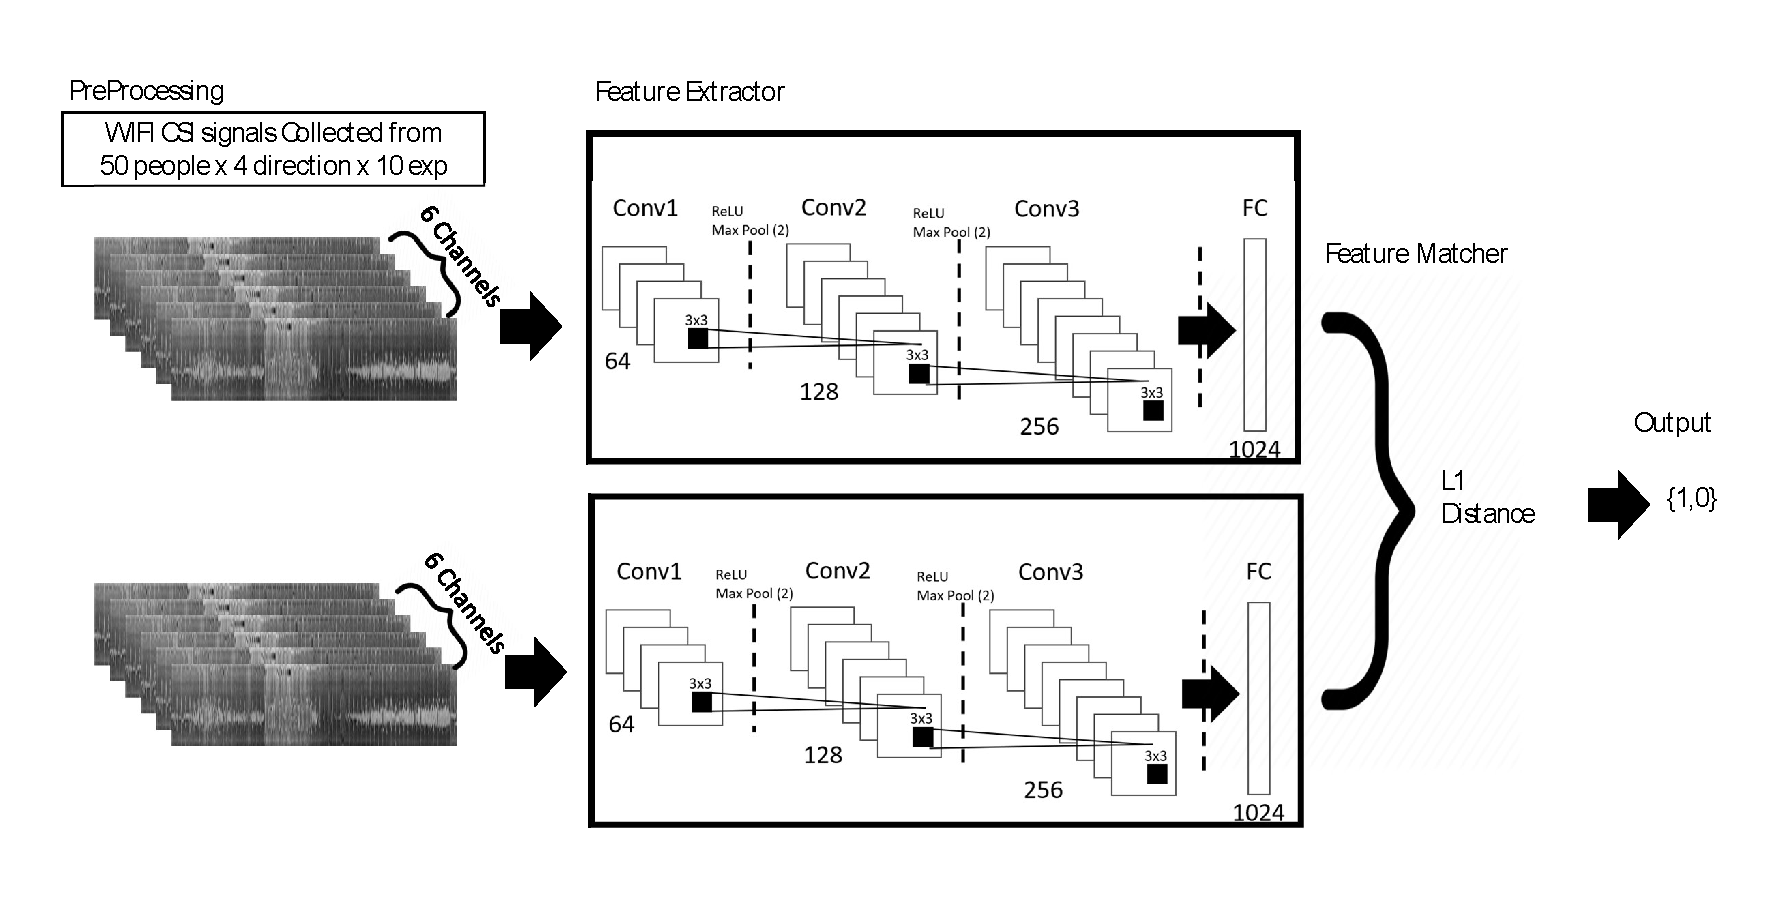
\includegraphics[width=\textwidth]{network1.eps}
\caption{...} \label{network1}
\end{figure}

\section{Experiments}
\section{Conclusion}

%
% ---- Bibliography ----
%
% BibTeX users should specify bibliography style 'splncs04'.
% References will then be sorted and formatted in the correct style.
%
% \bibliographystyle{splncs04}
% \bibliography{mybibliography}
%
\begin{thebibliography}{8}
\bibitem{ref_article1}
Koch, Gregory, Richard Zemel, and Ruslan Salakhutdinov.
 "Siamese neural networks for one-shot image recognition." 
 ICML deep learning workshop. Vol. 2. 2015.


\end{thebibliography}
\end{document}




%% Template End
\section{*** Template ***}
\section{First Section}
\subsection{A Subsection Sample}
Please note that the first paragraph of a section or subsection is
not indented. The first paragraph that follows a table, figure,
equation etc. does not need an indent, either.

Subsequent paragraphs, however, are indented.

\subsubsection{Sample Heading (Third Level)} Only two levels of
headings should be numbered. Lower level headings remain unnumbered;
they are formatted as run-in headings.

\paragraph{Sample Heading (Fourth Level)}
The contribution should contain no more than four levels of
headings. Table~\ref{tab1} gives a summary of all heading levels.

\begin{table}
\caption{Table captions should be placed above the
tables.}\label{tab1}
\begin{tabular}{|l|l|l|}
\hline
Heading level &  Example & Font size and style\\
\hline
Title (centered) &  {\Large\bfseries Lecture Notes} & 14 point, bold\\
1st-level heading &  {\large\bfseries 1 Introduction} & 12 point, bold\\
2nd-level heading & {\bfseries 2.1 Printing Area} & 10 point, bold\\
3rd-level heading & {\bfseries Run-in Heading in Bold.} Text follows & 10 point, bold\\
4th-level heading & {\itshape Lowest Level Heading.} Text follows & 10 point, italic\\
\hline
\end{tabular}
\end{table}


\noindent Displayed equations are centered and set on a separate
line.
\begin{equation}
x + y = z
\end{equation}
Please try to avoid rasterized images for line-art diagrams and
schemas. Whenever possible, use vector graphics instead (see
Fig.~\ref{fig1}).

\begin{figure}
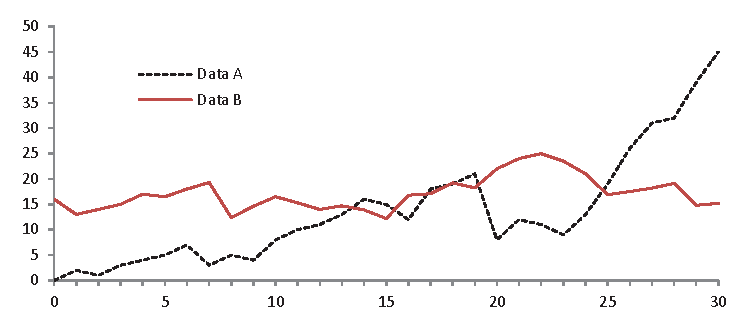
\includegraphics[width=\textwidth]{fig1.eps}
\caption{A figure caption is always placed below the illustration.
Please note that short captions are centered, while long ones are
justified by the macro package automatically.} \label{fig1}
\end{figure}

\begin{theorem}
This is a sample theorem. The run-in heading is set in bold, while
the following text appears in italics. Definitions, lemmas,
propositions, and corollaries are styled the same way.
\end{theorem}
%
% the environments 'definition', 'lemma', 'proposition', 'corollary',
% 'remark', and 'example' are defined in the LLNCS documentclass as well.
%
\begin{proof}
Proofs, examples, and remarks have the initial word in italics,
while the following text appears in normal font.
\end{proof}
For citations of references, we prefer the use of square brackets
and consecutive numbers. Citations using labels or the author/year
convention are also acceptable. The following bibliography provides
a sample reference list with entries for journal
articles~\cite{ref_article1}, an LNCS chapter~\cite{ref_lncs1}, a
book~\cite{ref_book1}, proceedings without editors~\cite{ref_proc1},
and a homepage~\cite{ref_url1}. Multiple citations are grouped
\cite{ref_article1,ref_lncs1,ref_book1},
\cite{ref_article1,ref_book1,ref_proc1,ref_url1}.
%
% ---- Bibliography ----
%
% BibTeX users should specify bibliography style 'splncs04'.
% References will then be sorted and formatted in the correct style.
%
% \bibliographystyle{splncs04}
% \bibliography{mybibliography}
%
\begin{thebibliography}{8}
\bibitem{ref_article1}
Author, F.: Article title. Journal \textbf{2}(5), 99--110 (2016)

\bibitem{ref_lncs1}
Author, F., Author, S.: Title of a proceedings paper. In: Editor,
F., Editor, S. (eds.) CONFERENCE 2016, LNCS, vol. 9999, pp. 1--13.
Springer, Heidelberg (2016). \doi{10.10007/1234567890}

\bibitem{ref_book1}
Author, F., Author, S., Author, T.: Book title. 2nd edn. Publisher,
Location (1999)

\bibitem{ref_proc1}
Author, A.-B.: Contribution title. In: 9th International Proceedings
on Proceedings, pp. 1--2. Publisher, Location (2010)

\bibitem{ref_url1}
LNCS Homepage, \url{http://www.springer.com/lncs}. Last accessed 4
Oct 2017
\end{thebibliography}
\end{document}
